% FEATHER — paper draft (v3: IEEE conference format, extended related work,
% full experimental results). Compiles on Overleaf with pdfLaTeX + BibTeX:
% main.tex + references.bib + figures/. Bibliography style: IEEEtranN (ships
% with the IEEEtran package on TeX Live and Overleaf).

\documentclass[conference]{IEEEtran}

\usepackage{amsmath,amssymb,amsthm}
\usepackage{graphicx}
\usepackage{booktabs}
\usepackage{microtype}
\usepackage{xcolor}
\usepackage{tikz}
\usetikzlibrary{arrows.meta,positioning}
\usepackage{algorithm}
\usepackage{algpseudocode}
\usepackage[numbers,sort&compress]{natbib}
\usepackage[colorlinks=true,linkcolor=blue,citecolor=blue,urlcolor=blue]{hyperref}

\newtheorem{proposition}{Proposition}
\newtheorem{assumption}{Assumption}
\newcommand{\todo}[1]{\textcolor{red}{[TODO: #1]}}

\newcommand{\R}{\mathbb{R}}
\newcommand{\E}{\mathbb{E}}
\newcommand{\F}{\mathbf{F}}
\newcommand{\act}{\phi}
\DeclareMathOperator{\rank}{rank}
\DeclareMathOperator{\spn}{span}
\DeclareMathOperator*{\softmax}{softmax}

\begin{document}

\title{FEATHER: Fisher-Eigenvalue Adaptive Thresholding\\for Error-Robust Drift Detection}

\author{%
  \IEEEauthorblockN{\todo{Author One}}
  \IEEEauthorblockA{\todo{Department, Institution}\\ \todo{City, Country}\\ \todo{email}}
  \and
  \IEEEauthorblockN{\todo{Author Two}}
  \IEEEauthorblockA{\todo{Department, Institution}\\ \todo{City, Country}\\ \todo{email}}
}

\maketitle

\begin{abstract}
Most practical tools for monitoring a deployed classifier without labels read
the model's outputs: softmax confidence, entropy, agreement statistics, or a
proxy trained to predict errors. We point out that this whole family shares a
blind spot that can be written down exactly. For a $C$-class softmax head, the
Fisher information of the log-likelihood with respect to the penultimate
activation has rank at most $C-1$; its orthogonal complement consists
precisely of the activation directions that shift every logit by the same
amount, and the softmax is invariant to such shifts. Data can therefore drift
arbitrarily far along these directions while confidence, entropy, and every
other output statistic stay frozen. FEATHER is a streaming monitor built
around this observation. A single pass over labeled reference data yields the
exact $d \times d$ Fisher matrix and its blind subspace; online monitoring
then costs one projection per batch, with thresholds calibrated by bootstrap
so the false-alarm rate is chosen rather than tuned. On a linear testbed the
implementation reproduces the theory to machine precision. On Rotated MNIST
and CIFAR-10-C (five seeds each) the blind-shift score tracks the measured
accuracy drop closely, the predicted rank structure appears exactly
($9$ informative directions out of $512$ in a ResNet-18, with a
fourteen-order-of-magnitude spectral gap), and against a covariance-based
ablation of itself the Fisher geometry cuts false alarms on benign episodes
almost in half (46\% vs.\ 80\% of batches at matched calibration).
\end{abstract}

\begin{IEEEkeywords}
concept drift, dataset shift, Fisher information, model monitoring,
label-free evaluation, machine learning systems
\end{IEEEkeywords}

\section{Introduction}

A model that was accurate at deployment does not stay accurate for free. The
data it sees keeps changing, and the change is only sometimes harmless. In
production systems this is not a corner case but a standing operational
burden --- Sculley et al.\ list undeclared data dependencies and changing
input distributions among the main sources of technical debt in machine
learning systems \citep{sculley2015debt} --- and monitoring for such
\emph{concept drift} is awkward for a simple reason: the labels that would
settle the question arrive late or never \citep{gama2014survey,
lu2018learning}. So the field has developed label-free proxies. Some watch
the input distribution and alarm on any change, which buries operators in
alerts about shifts the model tolerates perfectly well
\citep{rabanser2019failing}. The more recent and more useful family watches
the model's \emph{outputs} instead: confidence tracking
\citep{hendrycks2017baseline}, differences of confidences
\citep{guillory2021doc}, learned confidence thresholds \citep{garg2022atc},
prediction-uncertainty indices \citep{pudd2025}, and error-proxy models with
sequential testing \citep{amoukou2024sequential}.

Our starting point is a structural property of that second family. Whatever
is computed from the model's outputs is invariant to anything that leaves the
outputs unchanged. This sounds vacuous until one asks how much room ``leaves
the outputs unchanged'' actually describes. The answer, for a softmax
classifier, is: almost all of activation space. The Fisher information matrix
of the log-likelihood with respect to the penultimate activation $\act$ has
rank at most $C-1$, so for a ResNet-18 on CIFAR-10 the model's outputs are
sensitive to a $9$-dimensional slice of a $512$-dimensional feature space.
The remaining $503$ directions shift all logits equally; the softmax cancels
them; confidence and entropy do not move. If the world drifts along those
directions, the model cannot react, and neither can any monitor built on its
outputs. Failure, if it comes, is silent.

FEATHER (Fisher-Eigenvalue Adaptive Thresholding for Error-Robust drift
detection) watches exactly that region. Offline, one pass over a labeled
held-out set gives the Fisher matrix in closed form (it is only
$d \times d$, so no Kronecker or diagonal approximation is needed), an
eigendecomposition splits activation space into a sensitive and a blind
subspace, and bootstrap resampling of clean reference batches fixes alarm
thresholds at a chosen false-alarm rate. Online, each batch costs one
matrix--vector projection. A cascaded variant, FEATHER-Lite, puts a cheap
classical detector in front as a first stage and uses FEATHER to decide
whether a flagged shift is one the model's outputs can even see.

The paper makes three contributions.
\begin{enumerate}
  \item A two-line impossibility result
    (Proposition~\ref{prop:blind}): the blind subspace is exactly the set of
    softmax-invariant directions, so drift confined to it defeats every
    output-based monitor by construction, not by bad luck.
  \item The FEATHER monitor itself: exact offline computation, millisecond
    online cost, three complementary statistics, and thresholds calibrated to
    a chosen false-alarm budget.
  \item An evaluation on Rotated MNIST and CIFAR-10-C in which harmfulness is
    \emph{measured} from held-out labels rather than assumed from corruption
    names, including an ablation that isolates what the Fisher weighting adds
    over plain activation covariance, and an honest account of where standard
    corruption benchmarks stop being informative.
\end{enumerate}

\section{Related Work}
\label{sec:related}

\subsection{Drift detection as change detection}

Sequential change detection is old --- Page's CUSUM chart dates to 1954
\citep{page1954cusum} --- and the stream-mining literature adapted it to
learning systems as hypothesis tests on a running stream. DDM monitors the
classifier's error rate for significant increases \citep{gama2004learning},
EDDM refines it for gradual drift by tracking the distance between errors
\citep{baena2006eddm}, ADWIN compares adaptive sub-windows of a scalar
statistic \citep{bifet2007adwin}, and KSWIN applies a Kolmogorov--Smirnov
test on sliding windows \citep{raab2020kswin}; mature implementations of all
of these ship in the River library \citep{montiel2021river}. The error-rate
detectors are the right idea with the wrong input: they need labels, which is
exactly what streams lack. Surveys of the area
\citep{gama2014survey, lu2018learning} treat the label-scarcity problem as
central and unsolved.

Distribution-level alternatives drop the label requirement by testing whether
the inputs themselves changed, using kernel two-sample statistics such as MMD
\citep{gretton2012kernel} or classifier-based tests, with the general
taxonomy of covariate, label, and concept shift laid out in
\citep{quinonero2009dataset} and label-shift estimation treated in
\citep{lipton2018label}. These tests are performance-agnostic by design.
Rabanser et al.\ \citep{rabanser2019failing} made the resulting problem
concrete in an empirical study: detection strength and actual damage
correlate poorly, and characterizing \emph{harmful} shift was left open.
That gap is the one this paper addresses.

\subsection{Confidence, uncertainty, and label-free accuracy estimation}

A newer line asks the operational question directly: how well is the model
doing right now, without labels? The maximum-softmax-probability baseline
\citep{hendrycks2017baseline} started the trend of reading the answer off
the model's own confidence, and its descendants refine the readout: DoC
regresses accuracy on differences of confidences \citep{guillory2021doc},
ATC learns a confidence threshold whose exceedance rate estimates target
accuracy \citep{garg2022atc}, and PUDD detects drift early from prediction
uncertainty \citep{pudd2025}. Two well-known facts complicate the picture:
modern networks are systematically miscalibrated \citep{guo2017calibration},
and calibration degrades further precisely under the dataset shift one wants
to detect \citep{ovadia2019trust}. Closest to our setting, Amoukou et al.\
\citep{amoukou2024sequential} formalize sequential harmful-shift detection
without labels using an error proxy and sequential testing, and we adopt
their problem framing.

Every method in this paragraph, however, computes its signal from model
outputs or from a model trained to imitate them, and therefore inherits the
blind spot of Proposition~\ref{prop:blind}. We see them as complements: they
cover the drift the model can see, FEATHER covers the drift it cannot.

\subsection{Feature-space and out-of-distribution detection}

Working in the penultimate activation space is standard practice in
out-of-distribution detection: the Mahalanobis method
\citep{lee2018mahalanobis} scores individual samples against class-conditional
Gaussians fit to features, and Rabanser et al.'s strongest shift detector
(BBSD) also runs a test on model representations
\citep{rabanser2019failing}. What these methods lack is a criterion for
\emph{which} feature directions matter to the task: they weight feature space
by its variance or density, not by its effect on the model's decisions.
Benchmarks in this area, notably the common-corruptions suite
\citep{hendrycks2019benchmarking} that we also use, and the in-the-wild
shifts of WILDS \citep{koh2021wilds}, likewise do not distinguish shift the
model survives from shift that hurts it; we return to this point in
Section~\ref{sec:saturation}.

\subsection{Fisher geometry of neural networks}

The Fisher matrix enters deep learning mostly through optimization and
continual learning: natural gradient \citep{amari1998natural}, its KFAC
approximation \citep{martens2015kfac}, and Fisher-weighted regularization
against forgetting \citep{kirkpatrick2017overcoming}. Karakida et al.\
\citep{karakida2019universal} showed that deep-network Fisher spectra
concentrate in a handful of large eigenvalues over a near-zero bulk, which is
precisely the structure we exploit --- although in our activation-space
setting the split is not merely statistical but exact, with an algebraic rank
bound (Section~\ref{sec:blind}). Two works bring related geometry toward
monitoring. Zhang et al.\ \citep{zhang2023score} track the Fisher \emph{score
vector} with multivariate control charts; the score is a different object
(a per-sample gradient, requiring labels or their surrogate, in parameter
space), and their charts give a detection signal rather than a harmfulness
criterion. Zero-Direction Probing \citep{pandey2025zdp} studies null
directions of activations for representational drift in language models,
without a task-supervised Fisher matrix or any harmful/benign distinction.
FEATHER sits in the gap between \citep{amoukou2024sequential}, who have the
problem but not the geometry, and \citep{pandey2025zdp}, who have the
geometry but not the problem. Table~\ref{tab:positioning} summarizes the
landscape.

\begin{table}[t]
  \centering
  \caption{Where FEATHER sits. ``Blind region'' asks whether the method can
  respond to drift along softmax-invariant activation directions
  (Proposition~\ref{prop:blind}).}
  \label{tab:positioning}
  \begin{tabular}{@{}lccc@{}}
    \toprule
    family & labels & harm- & blind \\
           & online & aware & region \\
    \midrule
    error-rate charts (DDM, EDDM)          & yes & yes & --- \\
    input tests (MMD, KS, ADWIN)           & no  & no  & partly \\
    output-based (MSP, DoC, ATC, PUDD)     & no  & yes & no \\
    error proxies \citep{amoukou2024sequential} & no & yes & no \\
    feature density \citep{lee2018mahalanobis} & no & no & partly \\
    FEATHER (this work)                    & no  & yes & yes \\
    \bottomrule
  \end{tabular}
\end{table}

\section{Problem Setup}
\label{sec:setup}

Let $f(x) = \softmax(W\act(x) + b)$ be a deployed, frozen $C$-class
classifier with penultimate activation $\act(x) \in \R^d$,
$W \in \R^{C \times d}$, $b \in \R^C$. Batches $B_t$ arrive from a stream
without labels. A labeled held-out set $\{(\act_i, y_i)\}_{i=1}^{n}$ is
available once, offline. The task is to raise an alarm when the stream has
drifted in a way that plausibly degrades accuracy, while staying quiet under
drift the model tolerates --- and to do so, in particular, in the regime
where the model's own outputs carry no signal.

The one piece of structure everything below rests on is elementary: for any
$c \in \R$,
\begin{equation}
  \softmax(z + c\,\mathbf{1}) = \softmax(z),
  \label{eq:invariance}
\end{equation}
the softmax is invariant to shifting all logits together. Any activation
perturbation $u$ with $Wu \propto \mathbf{1}$ is therefore invisible in the
outputs, sample by sample.

\begin{figure}[t]
  \centering
  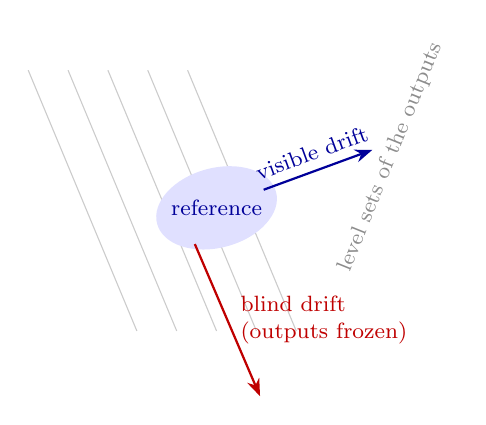
\begin{tikzpicture}[font=\small, scale=0.92,
      arrow/.style={-{Stealth[length=2.2mm]}, thick}]
    % logit level sets (lines of constant output)
    \foreach \i in {-1,0,1,2,3} {
      \draw[black!20] (-0.4 + 0.55*\i, -0.5) -- (-1.9 + 0.55*\i, 3.1);
    }
    \node[text=black!45, font=\footnotesize, rotate=68] at (2.55, 1.9)
      {level sets of the outputs};
    % reference cloud
    \fill[blue!12] (0.15,1.2) ellipse [x radius=0.85, y radius=0.55, rotate=15];
    \node[text=blue!60!black, font=\footnotesize] at (0.15,1.2) {reference};
    % visible drift: perpendicular to level sets
    \draw[arrow, blue!60!black] (0.8,1.45) -- (2.3,2.0)
      node[midway, above, sloped, font=\footnotesize] {visible drift};
    % blind drift: along level sets
    \draw[arrow, red!75!black] (-0.15,0.7) -- (0.75,-1.4)
      node[midway, right=1pt, font=\footnotesize, align=left]
      {blind drift\\(outputs frozen)};
  \end{tikzpicture}
  \caption{The geometry in caricature. The model's outputs are constant along
  their level sets in activation space; drift across level sets moves
  confidence and entropy, drift along them moves nothing the output can
  express. For a $C$-class softmax head the ``along'' directions form a
  $(d-C+1)$-dimensional subspace.}
  \label{fig:geometry}
\end{figure}

\section{The FEATHER Monitor}
\label{sec:method}

\subsection{The activation-space Fisher matrix and its blind subspace}
\label{sec:blind}

We take as monitoring object the empirical Fisher information of the
log-likelihood \emph{with respect to the activation},
\begin{equation}
  \F \;=\; \frac{1}{n}\sum_{i=1}^{n} g_i g_i^\top,
  \qquad
  g_i \;=\; \nabla_{\act}\log p(y_i \mid \act_i)
        \;=\; W^\top\!\big(e_{y_i} - p_i\big),
  \label{eq:fisher}
\end{equation}
with $p_i = \softmax(W\act_i + b)$ and $e_y$ the one-hot vector. Every $g_i$
lies in $W^\top\!\mathcal{H}$, where
$\mathcal{H} = \{v \in \R^C : \mathbf{1}^\top v = 0\}$ (the residual
$e_y - p$ sums to zero), so
\begin{equation}
  \rank \F \;\le\; \min\{\rank W,\; C-1\} \;\ll\; d .
  \label{eq:rank}
\end{equation}
$\F$ is $d \times d$ and computed exactly in one pass; the eigendecomposition
takes milliseconds. Writing $\lambda_1 \ge \dots \ge \lambda_d$ for its
eigenvalues with orthonormal eigenvectors $u_1,\dots,u_d$, we call
$\mathcal{S} = \spn\{u_j : \lambda_j > \tau\lambda_1\}$ the \emph{sensitive}
subspace and $\mathcal{N} = \mathcal{S}^\perp$ the \emph{blind} subspace. The
rank gap makes the split insensitive to $\tau$: in our ResNet-18 experiments
$\lambda_9/\lambda_1 \approx 5 \times 10^{-2}$ while
$\lambda_{10}/\lambda_1 \approx 10^{-16}$
(Fig.~\ref{fig:spectrum}), so any tolerance within fourteen orders of
magnitude gives the same answer. Fig.~\ref{fig:geometry} sketches the
resulting picture, and Fig.~\ref{fig:pipeline} the full pipeline.

\begin{figure*}[t]
  \centering
  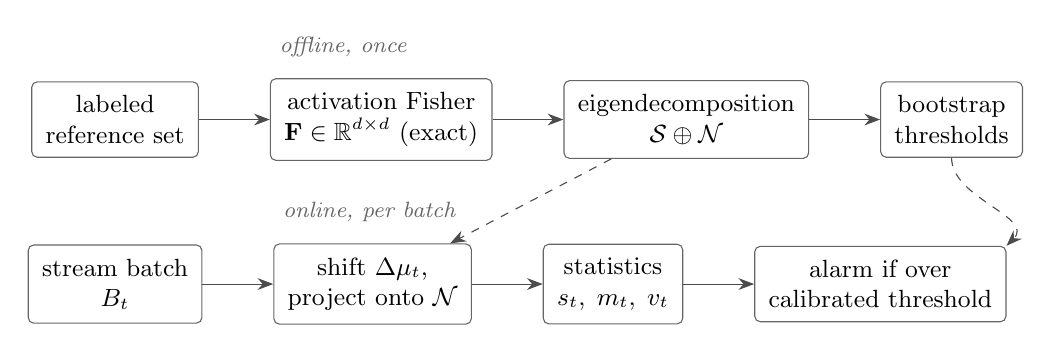
\begin{tikzpicture}[
      font=\small,
      box/.style={draw=black!60, rounded corners=2pt, minimum height=7mm,
                  inner sep=5pt, align=center},
      arrow/.style={-{Stealth[length=2mm]}, black!70},
      lab/.style={font=\footnotesize\itshape, text=black!60}
    ]
    % offline row
    \node[box] (ref) {labeled\\reference set};
    \node[box, right=9mm of ref] (fim) {activation Fisher\\$\F \in \R^{d\times d}$ (exact)};
    \node[box, right=9mm of fim] (eig) {eigendecomposition\\$\mathcal{S} \oplus \mathcal{N}$};
    \node[box, right=9mm of eig] (cal) {bootstrap\\thresholds};
    \draw[arrow] (ref) -- (fim);
    \draw[arrow] (fim) -- (eig);
    \draw[arrow] (eig) -- (cal);
    \node[lab, above=1.5mm of fim.north west, anchor=south west] {offline, once};
    % online row
    \node[box, below=11mm of ref] (batch) {stream batch\\$B_t$};
    \node[box, right=9mm of batch] (proj) {shift $\Delta\mu_t$,\\project onto $\mathcal{N}$};
    \node[box, right=9mm of proj] (stats) {statistics\\$s_t,\; m_t,\; v_t$};
    \node[box, right=9mm of stats] (alarm) {alarm if over\\calibrated threshold};
    \draw[arrow] (batch) -- (proj);
    \draw[arrow] (proj) -- (stats);
    \draw[arrow] (stats) -- (alarm);
    \draw[arrow, dashed] (eig) -- (proj);
    \draw[arrow, dashed] (cal.south) to[out=-90,in=45] (alarm.north east);
    \node[lab, above=1.5mm of proj.north west, anchor=south west] {online, per batch};
  \end{tikzpicture}
  \caption{The FEATHER pipeline. Everything expensive happens once, offline;
  the streaming side is a projection and three scalar comparisons.}
  \label{fig:pipeline}
\end{figure*}

\subsection{Online statistics}
\label{sec:stats}

Let $\mu_{\mathrm{ref}}$ be the reference activation mean and $B_\mathcal{N}$
an orthonormal basis of $\mathcal{N}$. For a batch with mean $\mu_t$ and
shift $\Delta\mu_t = \mu_t - \mu_{\mathrm{ref}}$ we track three numbers. The
direction ratio
\begin{equation}
  s_t = \frac{\lVert B_\mathcal{N}^\top \Delta\mu_t\rVert}
             {\lVert \Delta\mu_t\rVert}
\end{equation}
asks where the drift is pointing; a value near one means the movement is
almost entirely inside the blind subspace. The magnitude
$m_t = \lVert B_\mathcal{N}^\top \Delta\mu_t\rVert$ asks whether it is big
enough to matter --- $s_t$ alone is scale-invariant and would flag noise that
happens to point the wrong way. The energy
\begin{equation}
  v_t = \frac{1}{|B_t|}\sum_{x \in B_t}
        \big\lVert B_\mathcal{N}^\top(\act(x) - \mu_{\mathrm{ref}})\big\rVert^2
\end{equation}
catches drift that spreads into $\mathcal{N}$ without moving the mean.
Algorithm~\ref{alg:feather} puts the pieces together. The online cost is one
$d \times k$ projection per batch, where $k = \dim\mathcal{N}$.

\begin{algorithm}[t]
\caption{FEATHER}
\label{alg:feather}
\begin{algorithmic}[1]
\Statex \textbf{Offline} (once, labeled reference set):
\State compute $g_i = W^\top(e_{y_i} - p_i)$ and
       $\F = \frac{1}{n}\sum_i g_i g_i^\top$
\State eigendecompose $\F$; split at the rank gap into
       $\mathcal{S} \oplus \mathcal{N}$; store basis $B_\mathcal{N}$,
       reference mean $\mu_{\mathrm{ref}}$
\State bootstrap clean reference batches; set thresholds
       $\theta_m, \theta_v$ at the $(1-\alpha)$ quantile of $m, v$
\Statex \textbf{Online} (per unlabeled batch $B_t$):
\State $\Delta\mu_t \gets \mathrm{mean}_{x \in B_t}\,\act(x) - \mu_{\mathrm{ref}}$
\State compute $s_t, m_t, v_t$ from $B_\mathcal{N}^\top$ projections
\State \textbf{alarm} if $m_t > \theta_m$ or $v_t > \theta_v$;
       report $s_t$ as the blind fraction of the shift
\end{algorithmic}
\end{algorithm}

\subsection{Calibration}

Thresholds for $m_t$ and $v_t$ are quantiles of their bootstrap distribution
over clean reference batches, so the stationary false-alarm rate is a chosen
parameter, not a tuned constant. We use 500 bootstrap batches and the 99th
percentile throughout. Section~\ref{sec:calibration} reports a practical
lesson about which data the bootstrap should resample.

\subsection{FEATHER-Lite}

FEATHER answers a narrow question: is the drift somewhere the model's outputs
cannot follow? Classical detectors answer a cheaper one: did anything change?
FEATHER-Lite chains them. A statistical first stage (KSWIN or ADWIN on a
scalar activation summary, via River \citep{montiel2021river}) flags
candidate change-points with high sensitivity; FEATHER then classifies the
flagged shift as output-visible, where confidence-based triage applies, or
blind, where it is the only witness. Detectors that consume labels appear in
our experiments only as an upper-bound reference.

\section{Theory}
\label{sec:theory}

\begin{assumption}
\label{ass:span}
The reference gradients $\{g_i\}$ span $W^\top\!\mathcal{H}$. This holds
almost surely once $C$ generic samples are seen; empirically we observe the
full rank $C-1$ in every run.
\end{assumption}

\begin{proposition}[Detector blindness]
\label{prop:blind}
Under Assumption~\ref{ass:span},
\[
  \mathcal{N} \;=\; \{\, u \in \R^d \;:\; Wu \in \spn\{\mathbf{1}\} \,\},
\]
the set of softmax-invariant directions. Any drift that only translates
activations within $\mathcal{N}$ leaves the model's outputs pointwise
unchanged, and with them every monitoring statistic computed from outputs:
confidence, entropy, prediction histograms, DoC, ATC, uncertainty indices,
and error proxies trained on outputs.
\end{proposition}

\begin{proof}
$\mathcal{S} = \spn\{g_i\} = W^\top\!\mathcal{H}$ by the assumption, so
$u \in \mathcal{N}$ iff $(Wu)^\top v = 0$ for all $v \in \mathcal{H}$, i.e.\
iff $Wu \in \mathcal{H}^\perp = \spn\{\mathbf{1}\}$. For such $u$,
$W(\act + tu) + b = (W\act + b) + tc\,\mathbf{1}$ for some $c$, and by
\eqref{eq:invariance} the softmax is unchanged. Outputs are unchanged input
by input, hence so is any functional of them.
\end{proof}

\begin{proposition}[Calibrated response in the sensitive subspace]
\label{prop:bounded}
For any perturbation $\Delta \in \R^d$ and class $y$,
$\big|\log p(y \mid \act + \Delta) - \log p(y \mid \act)\big|
\le 2\lVert W\Delta \rVert_\infty$. The response to sensitive-subspace drift
is bounded and continuous in the shift; the response to blind-subspace drift
is exactly zero.
\end{proposition}

\begin{proof}
$\log p(y \mid \act) = z_y - \mathrm{logsumexp}(z)$ with $z = W\act + b$. The
linear term moves by at most $\lVert W\Delta\rVert_\infty$, and logsumexp is
$1$-Lipschitz in the $\ell_\infty$ norm. The blind case is
Proposition~\ref{prop:blind}.
\end{proof}

A caution about what this does and does not say.
Proposition~\ref{prop:blind} is an impossibility result for output-based
monitoring, not a guarantee that blind drift hurts. First-order geometry
cannot force errors; the danger of the blind region is precisely that the
model cannot respond there, so when the label function or the upstream
feature extractor changes along those directions, nothing in the output
stream says so. Whether blind-subspace movement actually accompanies damage
in deep networks is an empirical question, and Section~\ref{sec:experiments}
measures it rather than assuming it. The subspace itself is a property of
the frozen head; on retraining it is recomputed exactly, in seconds, and we
keep it fixed between retrainings rather than tracking it online (streaming
decompositions exist \citep{halko2011structure} but were not needed).

\section{Experiments}
\label{sec:experiments}

\subsection{Setup}

\paragraph{Models and training}
A small CNN (two convolutional blocks, $d = 128$) trained on MNIST with Adam
(learning rate $10^{-3}$, 5 epochs) to $99.00 \pm 0.05\%$ test accuracy, and
a CIFAR-adapted ResNet-18 ($3{\times}3$ stem, no max-pool, $d = 512$, 11.2M
parameters) trained on CIFAR-10 with SGD (learning rate 0.1, cosine schedule,
50 epochs, standard crop-and-flip augmentation) to $94.15 \pm 0.07\%$. Five
seeds per model; the seed fixes initialization, data order, and augmentation,
and every run is resumable from checkpoints with full RNG state.

\paragraph{Drift streams}
The MNIST test set rotated by $0^\circ$--$90^\circ$ in $15^\circ$ steps, and
CIFAR-10-C \citep{hendrycks2019benchmarking} (19 corruptions $\times$ 5
severities, plus the clean test set), streamed in batches of 500. An
\emph{episode} is one corruption-severity pair (or one angle) for one seed:
$96 \times 5 = 480$ CIFAR episodes and $7 \times 5 = 35$ MNIST episodes,
1{,}920 monitored batches per CIFAR seed.

\paragraph{Ground truth}
We label episodes by \emph{measured} accuracy drop against the clean episode
--- benign below 2 points, harmful above 10, gray between --- rather than by
corruption name. Under this rule the CIFAR episodes split 60 benign, 134
gray, 286 harmful. The data justify the caution: fog at severity 1 is
benign, fog at severity 5 costs over 30 points, and treating ``fog'' as one
condition would average the two into meaninglessness.

\paragraph{Detectors}
FEATHER; a covariance ablation of FEATHER (identical pipeline with $\F$
replaced by the activation covariance and the same blind dimension,
isolating the Fisher weighting); and the output-based baselines, mean
max-softmax confidence \citep{hendrycks2017baseline} and mean prediction
entropy. Episode scores are threshold-free changes relative to the clean
episode.

\paragraph{Hardware and reproducibility}
One workstation GPU (RTX 4500 Ada, 24 GB). Training a ResNet-18 seed takes
376 s; the MNIST model, 23 s. Every figure and table in this section is
regenerated by a script in the repository from the logged runs.

\subsection{A linear testbed where every answer is known}

Before the deep networks, we validate on two-dimensional two-Gaussian
streams whose Bayes boundary is known in closed form, so the sensitive and
blind directions have analytical values. The implementation recovers the
blind eigenvector to $|\cos| > 1 - 10^{-6}$; under a blind-direction shift
of four standard deviations, softmax outputs change by less than $10^{-10}$
per sample (Proposition~\ref{prop:blind}, numerically) while the calibrated
monitor flags 15 of 15 post-onset batches with $s_t > 0.95$; under a
sensitive-direction shift the same monitor stays at its noise floor
($\bar{s}_t < 0.2$, no alarms). The stationary alarm rate over 200 clean
batches stays within the calibrated budget. All 38 unit and integration
tests, including these, run in under a second on CPU.

\subsection{The predicted rank structure appears exactly}

Equation~\eqref{eq:rank} bounds the Fisher rank by $C - 1 = 9$.
Fig.~\ref{fig:spectrum} shows the measured spectra: in every one of the ten
runs, exactly nine eigenvalues sit above machine precision. For a
representative CIFAR-10 seed, $\lambda_9 = 9.1 \times 10^{-5}$ and
$\lambda_{10} = 5 \times 10^{-19}$, a collapse of fourteen orders of
magnitude, leaving a 503-dimensional blind subspace in a 512-dimensional
feature space ($119$ of $128$ for the MNIST CNN). The claim in the
introduction --- output-based monitors watch a 9-dimensional slice of a
512-dimensional space --- is in this sense not a metaphor. It also settles
the choice of blind dimension without a tuning knob: any threshold placed
anywhere in a fourteen-decade window yields the same subspace.

\begin{figure*}[t]
  \centering
  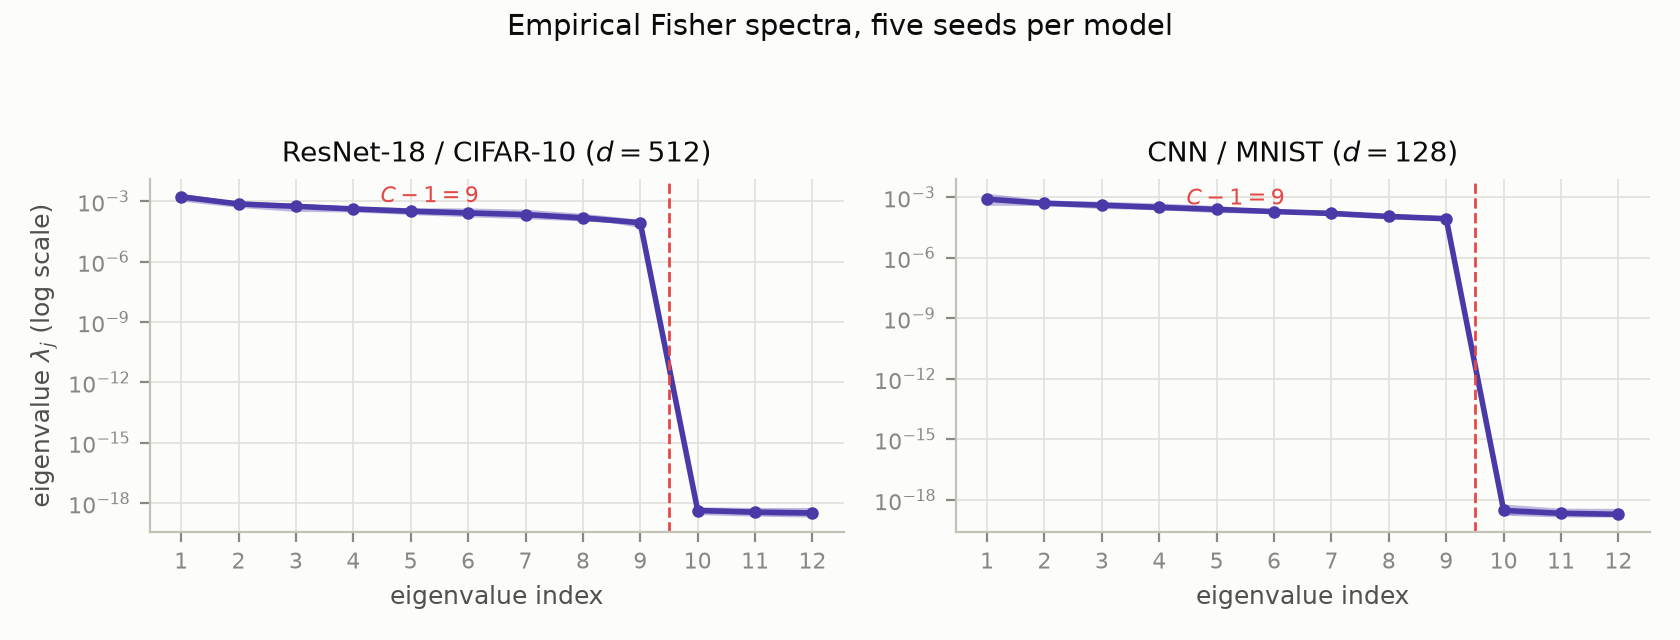
\includegraphics[width=0.86\linewidth]{figures/fisher_spectrum.png}
  \caption{Measured Fisher eigenvalue spectra for all five seeds of both
  models (thin lines: individual seeds; markers: mean). The spectrum
  collapses by fourteen orders of magnitude between index 9 and index 10,
  exactly at the algebraic bound $C - 1$ of \eqref{eq:rank}. The split into
  sensitive and blind subspaces is therefore parameter-free in practice.}
  \label{fig:spectrum}
\end{figure*}

\begin{figure*}[t]
  \centering
  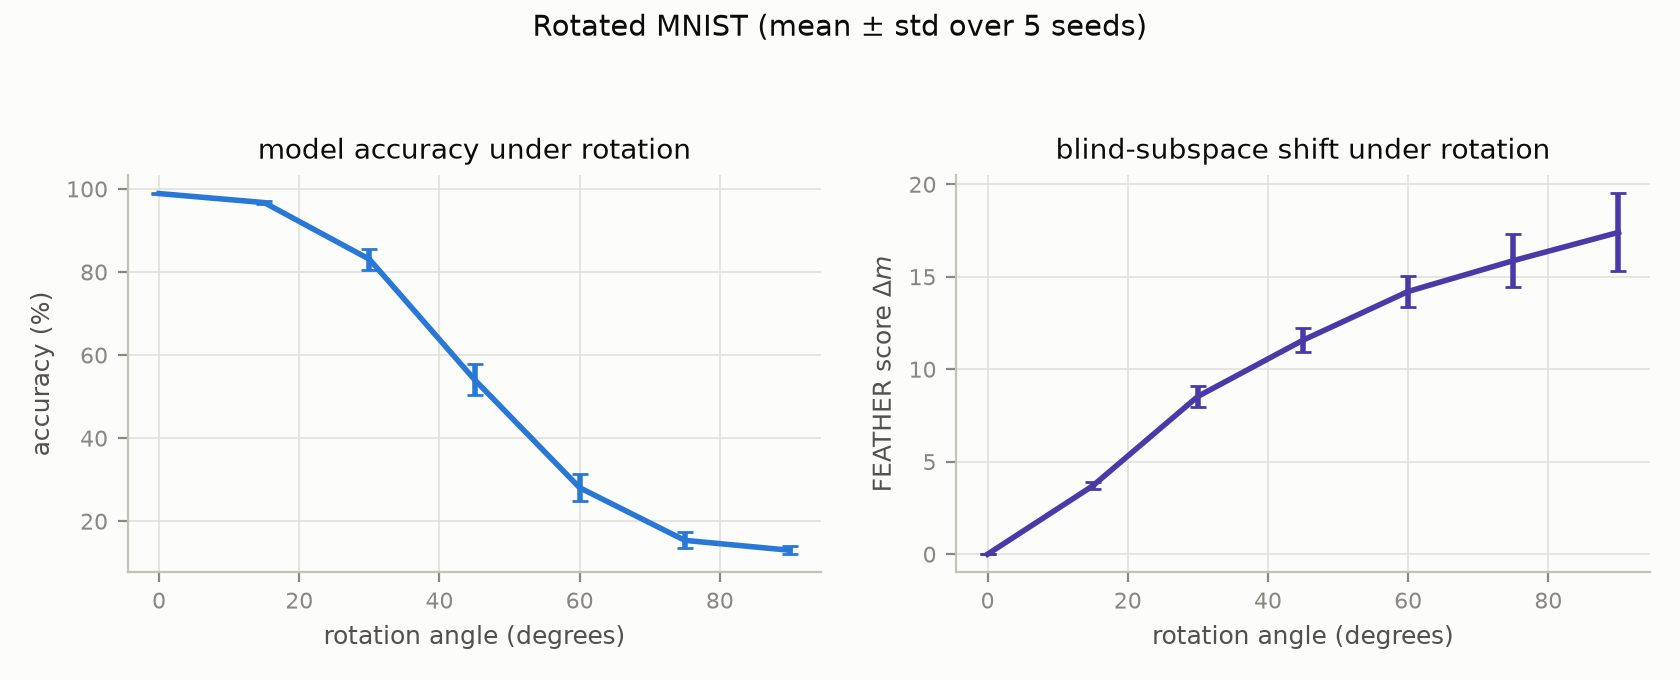
\includegraphics[width=0.86\linewidth]{figures/results_rotated_mnist.png}
  \caption{Rotated MNIST, mean $\pm$ std over five seeds. Accuracy falls
  smoothly with rotation angle (left) and the blind-subspace shift score
  rises with it (right), giving a monotone label-free proxy for the damage.}
  \label{fig:mnist}
\end{figure*}

\begin{figure}[t]
  \centering
  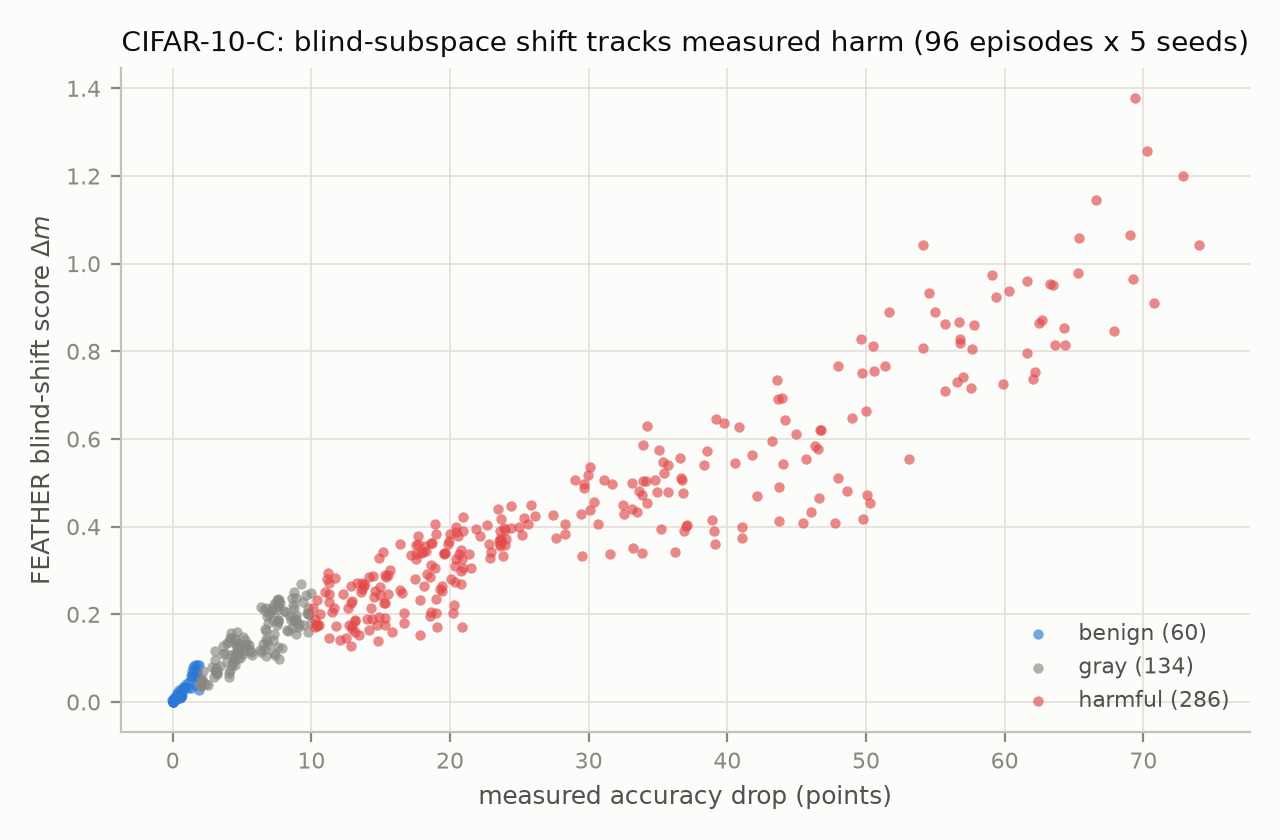
\includegraphics[width=\linewidth]{figures/results_cifar10c.png}
  \caption{CIFAR-10-C, all 96 episodes and five seeds (480 points). Each
  point is one episode; the blind-shift score grows with the measured
  accuracy drop across three orders of corruption severity.}
  \label{fig:cifar}
\end{figure}

\subsection{Blind-subspace shift tracks measured harm}

Fig.~\ref{fig:mnist} shows the Rotated MNIST sweep: accuracy decays from
99\% to 13\% as the angle grows, and the FEATHER score rises monotonically
with it. Fig.~\ref{fig:cifar} shows the same relationship on CIFAR-10-C at
the episode level: across 480 episode evaluations the blind-shift score and
the measured accuracy drop move together closely enough that the three harm
classes separate almost perfectly along the vertical axis.

\subsection{Where the benchmark stops discriminating}
\label{sec:saturation}

At the episode level this benchmark turns out not to discriminate between
detectors at all: harmful and benign episodes are separated with AUROC $1.0$
by FEATHER, by the covariance ablation, and by the confidence and entropy
baselines alike, on both benchmarks and every seed
(Table~\ref{tab:auroc}). We report this saturation rather than hiding it,
and draw the honest conclusion: standard corruption benchmarks produce
\emph{output-visible} drift, where output-based monitors work fine and
FEATHER matches them. This is consistent with the observation of
\citep{rabanser2019failing} that representation-level and output-level tests
all fire on synthetic corruptions; the benchmarks were built to be seen.
What separates the geometric methods is behavior under calibration, and what
separates FEATHER from its own covariance ablation is false alarms.

\begin{table}[t]
  \centering
  \caption{Episode-level AUROC (harmful vs.\ benign), mean over five seeds.
  Saturation across the board: corruption benchmarks generate drift every
  detector can see. The discriminating comparison is
  Table~\ref{tab:alarms}.}
  \label{tab:auroc}
  \begin{tabular}{@{}lcc@{}}
    \toprule
    detector & CIFAR-10-C & Rotated MNIST \\
    \midrule
    FEATHER              & 1.000 & 1.000 \\
    covariance ablation  & 1.000 & 1.000 \\
    confidence drop      & 1.000 & 1.000 \\
    entropy rise         & 1.000 & 1.000 \\
    \bottomrule
  \end{tabular}
\end{table}

\subsection{Fisher versus covariance: same pipeline, half the false alarms}

The ablation differs from FEATHER in one matrix. Both monitors use the same
blind dimension, the same bootstrap calibration at the 99th percentile, and
the same statistics; one projects onto the low-Fisher subspace, the other
onto the low-variance subspace of the activation covariance. On benign
CIFAR-10-C episodes --- where a specific monitor should stay quiet --- the
covariance monitor alarms on $79.7\%$ of batches, FEATHER on $45.8\%$; on
harmful episodes both alarm on every batch (Table~\ref{tab:alarms}).
Low-variance directions are apparently easy for benign corruptions to
excite; low-Fisher directions less so. The gap is the empirical content of
the Fisher weighting, and it answers the natural objection that the method
is PCA in disguise.

\begin{table}[t]
  \centering
  \caption{Batch-level alarm rates on CIFAR-10-C at matched calibration
  (99th-percentile bootstrap thresholds; five seeds). Both monitors catch
  every harmful batch; they differ on the benign episodes they should
  ignore. Both benign rates also reflect a calibration gap discussed in
  Section~\ref{sec:calibration}.}
  \label{tab:alarms}
  \begin{tabular}{@{}lcc@{}}
    \toprule
    & benign episodes & harmful episodes \\
    \midrule
    covariance ablation & 0.797 & 1.000 \\
    FEATHER             & \textbf{0.458} & 1.000 \\
    \bottomrule
  \end{tabular}
\end{table}

\subsection{A calibration finding}
\label{sec:calibration}

Bootstrap thresholds are calibrated on the same reference split that fits the
Fisher matrix, and this proves too optimistic: on MNIST even the unrotated
test set --- statistically the same distribution --- exceeds the calibrated
threshold, because the small train-to-test activation shift already has a
blind-subspace component larger than within-reference resampling predicts.
Episode-level conclusions are unaffected (all scores are computed relative to
the clean episode), but deployed thresholds should be calibrated on a clean
split held out from the Fisher fit. We flag this as a practical lesson the
controlled experiments would not have revealed, and note that it echoes the
general finding that uncertainty tooling degrades exactly where it is needed
\citep{ovadia2019trust}.

\subsection{Cost}

For the ResNet-18, the one-time offline fit --- activation extraction over
50{,}000 reference images, the exact Fisher matrix, eigendecomposition, and
500 bootstrap batches --- takes 11.2 s on the workstation GPU. Online
monitoring, including the forward pass, adds 47 ms per 500-image batch; the
projection itself is a $512 \times 503$ matrix--vector product, microseconds
of it. Monitoring is strictly cheaper than the inference it monitors, which
matters because a monitor that competes with serving for GPU time tends to
get switched off.

\section{Limitations}

The blind subspace is exact for the softmax head but summarizes deeper
feature drift only through the penultimate layer; a multi-layer variant via
Kronecker-factored parameter-space Fisher \citep{martens2015kfac} is a
natural extension. Proposition~\ref{prop:blind} says what output-based
monitors cannot see, not that blind drift must hurt; and pure concept shift
that leaves activation marginals untouched is invisible to every label-free
method, ours included. Our benchmarks, like most public corruption suites,
generate output-visible drift, so they exercise FEATHER's tracking and
false-alarm behavior but not the silent regime where
Proposition~\ref{prop:blind} gives it a monopoly; constructing realistic
silent-drift benchmarks --- perhaps from the wild shifts cataloged in WILDS
\citep{koh2021wilds} rather than synthetic corruptions --- is, we think, the
most valuable follow-up. Finally, thresholds should be calibrated on data
held out from the Fisher fit (Section~\ref{sec:calibration}).

\section{Conclusion}

Label-free monitoring has converged on reading the model's outputs, and the
geometry of a softmax head makes the cost of that choice precise: the outputs
are a $(C-1)$-dimensional window onto a $d$-dimensional representation, and
everything orthogonal to the window is invisible. FEATHER computes the
invisible part exactly, watches it for the price of a projection, and in
experiments tracks measured damage while halving the false alarms of its own
covariance ablation. The monitor is not a replacement for confidence-based
tools; it is the complement that covers the one region they provably cannot.

\bibliographystyle{IEEEtranN}
\bibliography{references}

\end{document}
